\documentclass{article}
\usepackage[UTF8]{ctex}
\usepackage{geometry}
\usepackage{multirow}
\usepackage{natbib}
\geometry{left=3.18cm,right=3.18cm,top=2.54cm,bottom=2.54cm}
\usepackage{graphicx}
\pagestyle{plain}	
\usepackage{setspace}
\usepackage{enumerate}
\usepackage{caption2}
\usepackage{datetime} %日期
\renewcommand{\today}{\number\year 年 \number\month 月 \number\day 日}
\renewcommand{\captionlabelfont}{\small}
\renewcommand{\captionfont}{\small}
\begin{document}

\begin{figure}
    \centering
    
\includegraphics[width=8cm]{upc.png}

    \label{figupc}
\end{figure}

	\begin{center}
		\quad \\
		\quad \\
		\heiti \fontsize{45}{17} \quad \quad \quad 
		\vskip 1.5cm
		\heiti \zihao{2} 《计算科学导论》个人职业规划
	\end{center}
	\vskip 2.0cm
		
	\begin{quotation}
% 	\begin{center}
		\doublespacing
		
        \zihao{4}\par\setlength\parindent{7em}
		\quad 

		学生姓名:\underline{\qquad  张三 \qquad \qquad}

		学\hspace{0.61cm} 号:\underline{\qquad 190701xxxx\qquad}
		
		专业班级:\underline{\qquad 计科1901 \qquad  }
		
        学\hspace{0.61cm} 院:\underline{计算机科学与技术学院}
% 	\end{center}
		\vskip 1.5cm
		\centering
		\begin{table}[h]
            \centering 
            \zihao{4}
            \begin{tabular}{|c|c|c|c|c|c|c|c|c|}
            % 这里的rl 与表格对应可以看到,姓名是r,右对齐的;学号是l,左对齐的;若想居中,使用c关键字。
                \hline
                \multicolumn{5}{|c|}{分项评价} &\multicolumn{2}{c|}{整体评价}  & 总    分 & 评 阅 教 师\\
                \hline
                自我 & 环境 & 职业 & 实施 & 评估与 & 完整性 & 可行性 &\multirow{2}*{} &\multirow{2}*{}\\
                分析& 分析& 定位 & 方案 & 调整 & 20\% & 20\% & ~&~ \\\            
                10\% & 10\% & 15\% & 15\% & 10\% & &  &~ &~\\
                \cline{1-7} 
                & & & & & & & ~&~ \\
                & & & & & & & ~&~ \\
                \hline      
            \end{tabular}
        \end{table}
		\vskip 2cm
		\today
	\end{quotation}

\thispagestyle{empty}
\newpage
\setcounter{page}{1}
% 在这之前是封面,在这之后是正文
\section{自我分析}
	自我分析即对自己进行全方位、多角度的分析,目的是认识自己、了解自己。只有认识了自己,才能对自己的职业做出正确的选择,才能选定适合自己发展的职业生涯路线,才能对自己的职业生涯目标做出最佳抉择。\par
	自我分析包括:\par
\subsection{自然条件}
性别、年龄、身体条件、健康状况、居住城市等。\par
\subsection{性格分析}
\par
\subsection{教育与学习经历}
\par
\subsection{工作与社会阅历}
\par
\subsection{知识、技能与经验}
\par
\subsection{兴趣爱好与特长}
\par
\section{环境分析}
环境分析主要是评估周边各种环境因素对自己职业生涯发展的影响。每一个人都处在一定的环境之中,职业发展必然要受到所处环境的影响,只有充分了解和把握所处环境的现状、特点、发展变化趋势,才能做到在复杂的环境中避害趋利,使你的职业生涯规划具有实际意义。\par
环境分析包括:\par
\subsection{社会环境分析}
政治形势、经济形势、就业形势等。\par
\subsection{家庭环境分析}
婚姻状况、经济状况、家人期望、家族传统等。\par
\subsection{职业环境分析}
行业现状及发展趋势;职业的工作内容、工作要求、发展前景等。\par


\subsection{地域与人际环境分析}
工作城市的气候水土、文化特点、发展前景;人脉与人际关系等。\par
\par 
图片插入的样例:\par
\begin{figure}[h!]
\centering
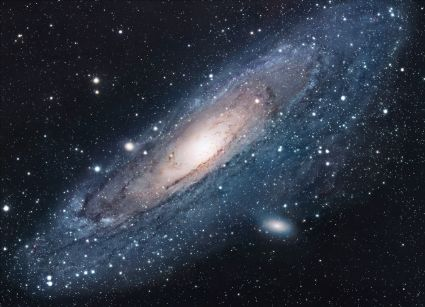
\includegraphics[scale=1.7]{universe}
\caption{The Universe}
\label{fig:universe}
\end{figure}



\section{职业定位}
在准确地对自己和环境做出了分析之后,确定适合自己行业和有实现可能的职业发展目标。职业定位时要注意与自己的自然条件、知识背景、技能特长、性格特点、兴趣爱好是否匹配,考虑与自己所处的环境是否相适应。职业定位决定了职业发展中的行为和结果,是制定职业生涯规划的关键,应当科学合理,具有可行性。\par
职业定位包括:\par

\subsection{行业领域定位与理由}
\par
\subsection{职业岗位起点定位与理由}
\par
\subsection{职业目标与可行性分析}
\par
成果目标、经济目标、能力目标、职务目标等。\par 
\begin{enumerate}[(1)]
	\item 短期目标(大学4年)
	\item 中长期目标(5-10年)。
\end{enumerate}
这里是简单列表的样例:(如果需要标号自定义或者自动标记数字序号,请自行搜索语法)
\begin{itemize}
    \item 简单的列表结构 
    \item 如这里所示
    \item 此处仅为样例
    \item 按需修改和使用
\end{itemize}


\section{实施方案}
在明确了职业定位后,要制定实现职业生涯目标的行动方案,不付诸行动,职业目标只能是一种梦想。实施方案是实现职业目标的保证,尽量考虑周全、具有可操作性。\par
实施方案可以从以下角度考虑:\par
\begin{enumerate}[1、]
	\item 如何利用现有条件和自身优势以实现职业生涯目标。
	\item 如何克服缺点、弥补不足、增长知识、提高能力以实现职业生涯目标。
	\item 如何处理人际关系和发展人脉以实现职业生涯目标。
	\item 如何处理工作与家庭、生活的关系以实现职业生涯目标。
	\item 如何处理释放工作压力、保证身心健康以实现职业生涯目标。
\end{enumerate}
\par 
表格插入样例(三线表):\par
%单元格怎么写?参考第一页打分的表格

\begin{table}[h]
	\centering
	\caption{这是科学系的花名册}
	\begin{tabular}{rl}
		% 这里的rl 与表格对应可以看到,姓名是r,右对齐的;学号是l,左对齐的;若想居中,使用c关键字。
		\hline
		姓名 & 学号 \\
		\hline
		张三 & 190704xxxx+++ \\ 
		李四 & 190704yyyy \\
		王二五 & 190704zzzz\\
		\hline
	\end{tabular}
	\label{table1}
\end{table}
\section{评估与调整}
由于影响职业生涯规划的因素很多,且大都处于动态变化之中,因此职业生涯规划应定期评估,并根据影响因素的变化和实施结果的情况及时作出调整,这样才能保证其行之有效。\par 
\subsection{评估时间}
可以选择每学期评估一次、每学年一次、三年评估一次。\par
\subsection{评估内容}
可以从成果目标、经济目标、能力目标、职务目标等方面总结,确定哪些目标已按预期实现,哪些目标商未达到,对已实现的成果总结经验,对未完成的目标分析原因。\par
\subsection{调整原则}
应考虑与自身情况的匹配性、与环境的适应性、操作实施的可行性等。\par




\end{document}
